\documentclass{article}

% if you need to pass options to natbib, use, e.g.:
%     \PassOptionsToPackage{numbers, compress}{natbib}
% before loading neurips_2018

% ready for submission
% \usepackage{neurips_2018}

% to compile a preprint version, e.g., for submission to arXiv, add add the
% [preprint] option:
%     \usepackage[preprint]{neurips_2018}

% to compile a camera-ready version, add the [final] option, e.g.:
     \usepackage[final]{neurips_2018}

% to avoid loading the natbib package, add option nonatbib:
%     \usepackage[nonatbib]{neurips_2018}

\usepackage[utf8]{inputenc} % allow utf-8 input
\usepackage[T1]{fontenc}    % use 8-bit T1 fonts
\usepackage{hyperref}       % hyperlinks
\usepackage{url}            % simple URL typesetting
\usepackage{booktabs}       % professional-quality tables
\usepackage{amsfonts}       % blackboard math symbols
\usepackage{nicefrac}       % compact symbols for 1/2, etc.
\usepackage{microtype}      % microtypography
\usepackage{amsmath}
\usepackage{amssymb}
\usepackage{graphicx}

\title{Variational Inference}

% The \author macro works with any number of authors. There are two commands
% used to separate the names and addresses of multiple authors: \And and \AND.
%
% Using \And between authors leaves it to LaTeX to determine where to break the
% lines. Using \AND forces a line break at that point. So, if LaTeX puts 3 of 4
% authors names on the first line, and the last on the second line, try using
% \AND instead of \And before the third author name.

\author{%
  Zhuoyuan Chen\thanks{}\\%Use footnote for providing further information
    %about author (webpage, alternative address)---\emph{not} for acknowledging
    %funding agencies.} \\
  Facebook AI Research\\
  Menlo Park, CA 94025 \\
  \texttt{chenzhuoyuan07@gmail.com} \\
  % examples of more authors
  % \And
  % Coauthor \\
  % Affiliation \\
  % Address \\
  % \texttt{email} \\
  % \AND
  % Coauthor \\
  % Affiliation \\
  % Address \\
  % \texttt{email} \\
  % \And
  % Coauthor \\
  % Affiliation \\
  % Address \\
  % \texttt{email} \\
  % \And
  % Coauthor \\
  % Affiliation \\
  % Address \\
  % \texttt{email} \\
}

\begin{document}
% \nipsfinalcopy is no longer used

\maketitle

\begin{abstract}
VI, VB, EM Summary
\end{abstract}

\section{Summary}
Given $\theta$ as parameter, $x$ observed, $z$ latent variables, we have
\begin{eqnarray}
l(\theta; D) = \log p(x)&=& \log\sum_z p(z|\theta) p(x|z, \theta)\\
&=&  \log\sum_z p(z|\theta) p(x|z, \theta)\frac{q(z)}{q(z)}\\
&=&\log\mathbb{E}_z\frac{p(x|z)p(z)}{q(z)}
\end{eqnarray}
According to Jensen's Inequality (log is concave), we have
\begin{eqnarray}
l(\theta; D) &=&\log p(z) =\log\sum_z q(z) \frac{p(x|\theta)}{q(z)}\\
&\ge& \sum_z q(z)  \log\frac{p(x|\theta)}{q(z)}\\
&=& \mathbb{E}_{z\sim q(z)} [\log p(x|z)+\log p(z)]-H(q)=\mathbb{E}_q\log p(x|z) - KL(q||p)
\end{eqnarray}
The evidence lower-bound (\textbf{ELBO}) is called free energy. The equality satisfies when $q(z|x) = p(z|x,\theta)$.  The difference between the gap is:
\begin{equation}
\log p(x) - ELBO = KL(q(z), p(z|x))
\end{equation}

\subsection{Application 1: GMM}
\begin{equation}
\log p(\theta; D)\ge \sum_z q(z|x)  \log\frac{p(x|\theta)}{q(z|x)}
\end{equation}
E-step:
\begin{equation}
q^{t+1} = \arg\max_q F(q, \theta^t)
\end{equation}
M-step:
\begin{equation}
\theta^{t+1} = \arg\max_{\theta} F(q^{t+1}, \theta)
\end{equation}

\begin{figure}
	\begin{center}
		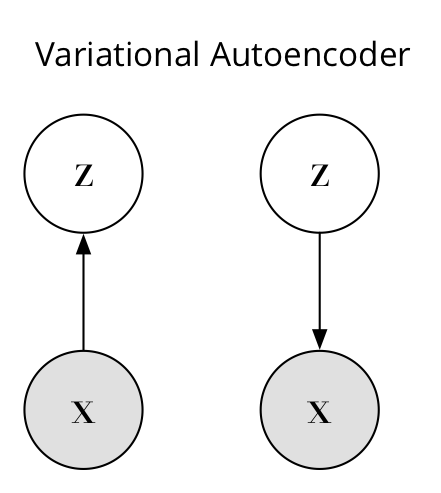
\includegraphics[width=.3\linewidth]{vae.png}
	\end{center}
	\caption{VAE.}
\label{fig-VAE}
\end{figure}

\subsection{Application 2: VAE}
Graphical model can be shown in Figure \ref{fig-VAE}. Traditional VI process:
\begin{enumerate}
\item Calculate $\nabla_\theta L_i(p,q_i)$ by
  \begin{enumerate}
    \item Sample $z\sim q_i(x_i)$
    \item $\nabla_{\theta}L_i(p,q_i)\approx \nabla_{\theta}\log p_{\theta}(x_i|z)$
  \end{enumerate}
\item $\theta \leftarrow \theta + \alpha\nabla_{\theta}L_i(p,q_i)$
\item update $q_i$ to maximize $L_i(p, q_i)$
\end{enumerate}
Each $q_i$ is different. So, the number of parameters is $|\theta|+(|\mu_i|+|\sigma_i|)\times N$, and step 3 is intractable. Using a neural network for $q(z_i)=q_{\phi}(x_i)$ makes the number of parameters independent of sample points. (This step is called \textbf{Amortized Variational Inference}). Then step 3 becomes:
\begin{equation*}
\phi \leftarrow \phi + \alpha\nabla_{\phi}L_i(p,q_i)
\end{equation*}
Learn by PG versus reparametrization trick:
\begin{eqnarray}
J(\phi) &\approx& \frac{1}{M}\nabla_{\phi}\log q_{\phi}(z|x)r(x_i, z_i)\\
&& \frac{1}{M} \nabla_{\phi}r(x_i, \mu_i+\sigma_i*\epsilon)
\end{eqnarray}
The second one has lower variance since it makes use of derivative of $r(x,z)$.

Encoder: $z = q(\phi,x)$, decoder: $x=p(\theta,z)$. We have MLE:
\begin{eqnarray}
KL(q(z|x), p(z|x)) & = & E_{q(z|x)}\log q(z|x) -  E_{q(z|x)}(\log P(x|z) + \log p(z) - \log p(x)) \\
E_{q(z|x)}\log p(x) &=& E_q \log p(x|z) - KL(q(z|x), p(z)) + KL(q(z|x), p(z|x))\\
 &=& ELBO + KL(q(z|x), p(z|x))
\end{eqnarray}
and loss to optimize is:
\begin{equation}
l(\phi, \theta) = -E_{x\sim q(x|z)} \log p(x|z) + KL(q(z|x), p(z))
\end{equation}

\subsection{Semi-Supervised VAE}
\begin{figure}
	\begin{center}
		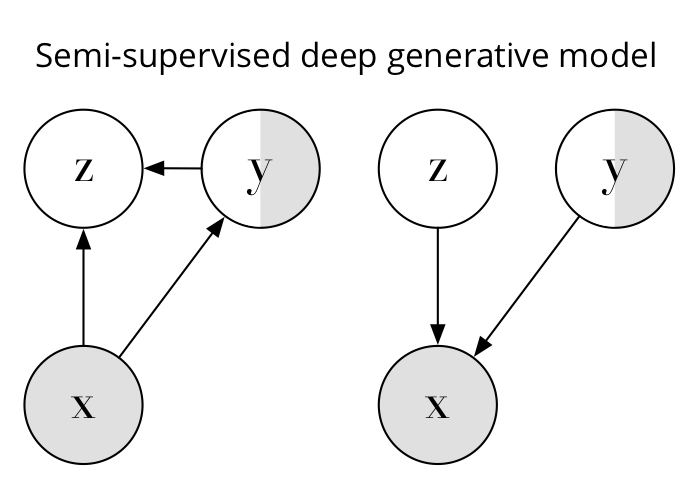
\includegraphics[width=.3\linewidth]{dgm.png}
	\end{center}
	\caption{Semi-supervised VAE.}
\label{fig-SSVAE}
\end{figure}

Graphical model can be shown in Figure \ref{fig-SSVAE}.
\begin{enumerate}
\item Label $y$ is known:
\begin{equation*}
\log p_{\theta}(x,y)\ge\mathbb{E}_{q_{\phi}(z|x,y)}[\log p_{\theta}(x|y,z)+\log p_{\theta}(y)+\log p(z)-\log q_{\phi}(z|x,y)]=-L(x,y)
\end{equation*}
\item Label $y$ is unknown:
\begin{eqnarray*}
\log p_{\theta}(x)&=&\log\sum_y\int_z q(z,y|x)\frac{p(x,y,z)}{q(z,y|x)}dz \ge \sum_y q(y|x)\int_z q(z|x,y)\log\frac{p(x,y,z)}{q(z,y|x)}dz\\
&=&\sum_y q(y|x)(-L(x,y)) + H(q(y|x))
\end{eqnarray*}
\end{enumerate}

\subsection{DVIB}
Graphical model: Y - X - Z, with cost function:
\begin{equation}
\arg\max_{\theta}I(Z,Y;\theta)-\beta I(Z,X;\theta)
\end{equation}
Then, the graphical model is:
\begin{equation*}
p(X,Y,Z)=p(X)p(Z|X)p(Y|X)
\end{equation*}
\begin{enumerate}
\item Lower bound of $I(Z;Y)$, with approximation $q_1(y|z)$:
\begin{equation*}
I(Z,Y)\ge\int p(y,z)\log\frac{q(y|z)}{p(y)} dy dz=\int p(y,z)\log q_1(y|z)  dy dz+ H(Y)
\end{equation*}
where we can drop $H(Y)$, using graphical model $p(x,y,z)=p(x)p(y|x)p(z|x)$, then we have:
\begin{equation*}
I(Z,Y)\ge\int p(x)p(y|x)p(z|x)\log q_1(y|z) dx dy dz
\end{equation*}
\item Upper bound of $I(X;Y)$, with approximation $q_2(z)$:
\begin{equation*}
I(Z,X)=\int p(x,z)\log\frac{p(z|x)}{p(z)}dz dx = \int p(x,z)\log p(z|x)dz dx - \int p(x,z)\log p(z)dz dx
\end{equation*}
Then, we have
\begin{equation*}
I(Z,X)\le \int p(x)p(z|x)\log\frac{p(z|x)}{q_2(z)}
\end{equation*}

\end{enumerate}

\section{Fisher Information Matrix, Natural Gradient}
\subsection{KL-Divergence}
\begin{eqnarray*}
&KL(p_w(x), p_{w+\triangle w}(x)) \\
=& E_{x\sim p_w(x)} \log p_w(x) - \log p_{w+\triangle w}(x)\\
=& E_{x\sim p_w(x)} \{\log p_w(x) - [\log p_w(x)+\nabla_w \log p_w(x)\triangle w + \frac{1}{2}\triangle w^T \nabla^2_w \log p_w(x)\triangle w)]\} \\
=& [E_{x\sim p_w(x)}\nabla_w \log p_w(x)]\triangle w -  \frac{1}{2}\triangle w^T [E_{x\sim p(x)}\nabla^2_w \log p_w(x)]\triangle w\\
= & \frac{1}{2}\triangle w[E_{x\sim p(x)}\nabla_w \log p_w(x)\nabla_w \log p_w(x)^T]\triangle w^T
\end{eqnarray*}
where
\begin{eqnarray*}
\nabla^2_w \log p_w(x) = \frac{\nabla^2_w p_w(x)}{p_w(x)} - \frac{\nabla_w p_w(x)\nabla_w p_w(x)^T}{p_w^2(x)} \\
= \frac{\nabla^2_w p_w(x)}{p_w(x)} - \nabla_w \log p_w(x)\nabla_w \log p_w(x)^T
\end{eqnarray*}
Also, we use the following property:
\begin{eqnarray*}
E_{x\sim p_w(x)}\nabla_w \log p_w(x) &=& \int_x p_w(x)\nabla_w \log p_w(x)dx=\int_x \nabla_w p_w(x)dx\\
&=&\nabla_w(\int_x  p_w(x)dx) = 0\\
E_{x\sim p_w(x)}\nabla^2_w \log p_w(x) &=& 0
\end{eqnarray*}
\subsection{Fisher-Information Matrix}
\begin{equation*}
E_{x\sim p(x)}\nabla_w \log p_w(x)\nabla_w \log p_w(x)^T
\end{equation*}

\section{Mutual Information}
In probability theory and information theory, the mutual information (MI) of two random variables is a measure of the mutual dependence between the two variables:
\begin{equation}
I(x;y) := KL(p_{x,y}, p_x \otimes p_y) = h(x) - h(x|y)\ge 0
\end{equation}
Intuitively, mutual information measures the information that $X$ and $Y$ share: It measures how much knowing one of these variables reduces uncertainty about the other.
Properties:
\begin{eqnarray}
I(X;Y)\ge 0\\
I(X;Y) = I(Y;X)\\
I(X;Y) = H(X) - H(X|Y) = H(Y) - H(Y|X) = \\
H(X)+H(Y)-H(X,Y) = H(X,Y)-H(X|Y)-H(Y|X)\\
I(X;Y)=\mathbb{E}_Y[KL(p_{x|y}, p_x)]
\end{eqnarray}
\end{document}
